\documentclass[a4paper,10pt]{article}
\usepackage{My_math_package}

\title{MATH808K - Algebraic K-Theory} % password: 
\author{Haoran Li}
\date{2020 Spring}

\makeindex[columns=2, title=Index, intoc] % Create the index

\begin{document}\sloppy % Reduce overlong words

% Maketitle
\begin{titlepage}
\begin{center}
\vspace*{1cm}
\Huge
\textbf{MATH808K - Algebraic K-Theory} \\
\vspace{2cm}
\begin{center}
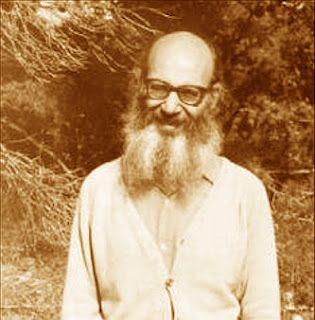
\includegraphics{Pictures/Grothendieck.jpg}
\end{center}
\vspace{2cm}
\normalsize
Taught by \texttt{Jonathan Rosenberg} \\
Notes taken by \texttt{Haoran Li} \\
2021 Spring \\
\vspace{2cm}
Department of Mathematics\\
University of Maryland\\
\end{center}
\end{titlepage}

% Contents
\tableofcontents
\newpage

\subfile{old.tex}
\begin{thebibliography}{}

\bibitem{Weibel} 
\textit{The K-Book} - Charles Weibel

\end{thebibliography}

\printindex
\newpage

\end{document}